\documentclass[border=20pt]{standalone}


\usepackage{pgfplots}
\usepackage{tikz}
\usepackage{pdfpages}
\usepackage{subfigure}
\usepackage{graphicx}

\begin{document}
%\definecolor{darkgreen)}{rgb}{0.0, 0.5, 0.0}
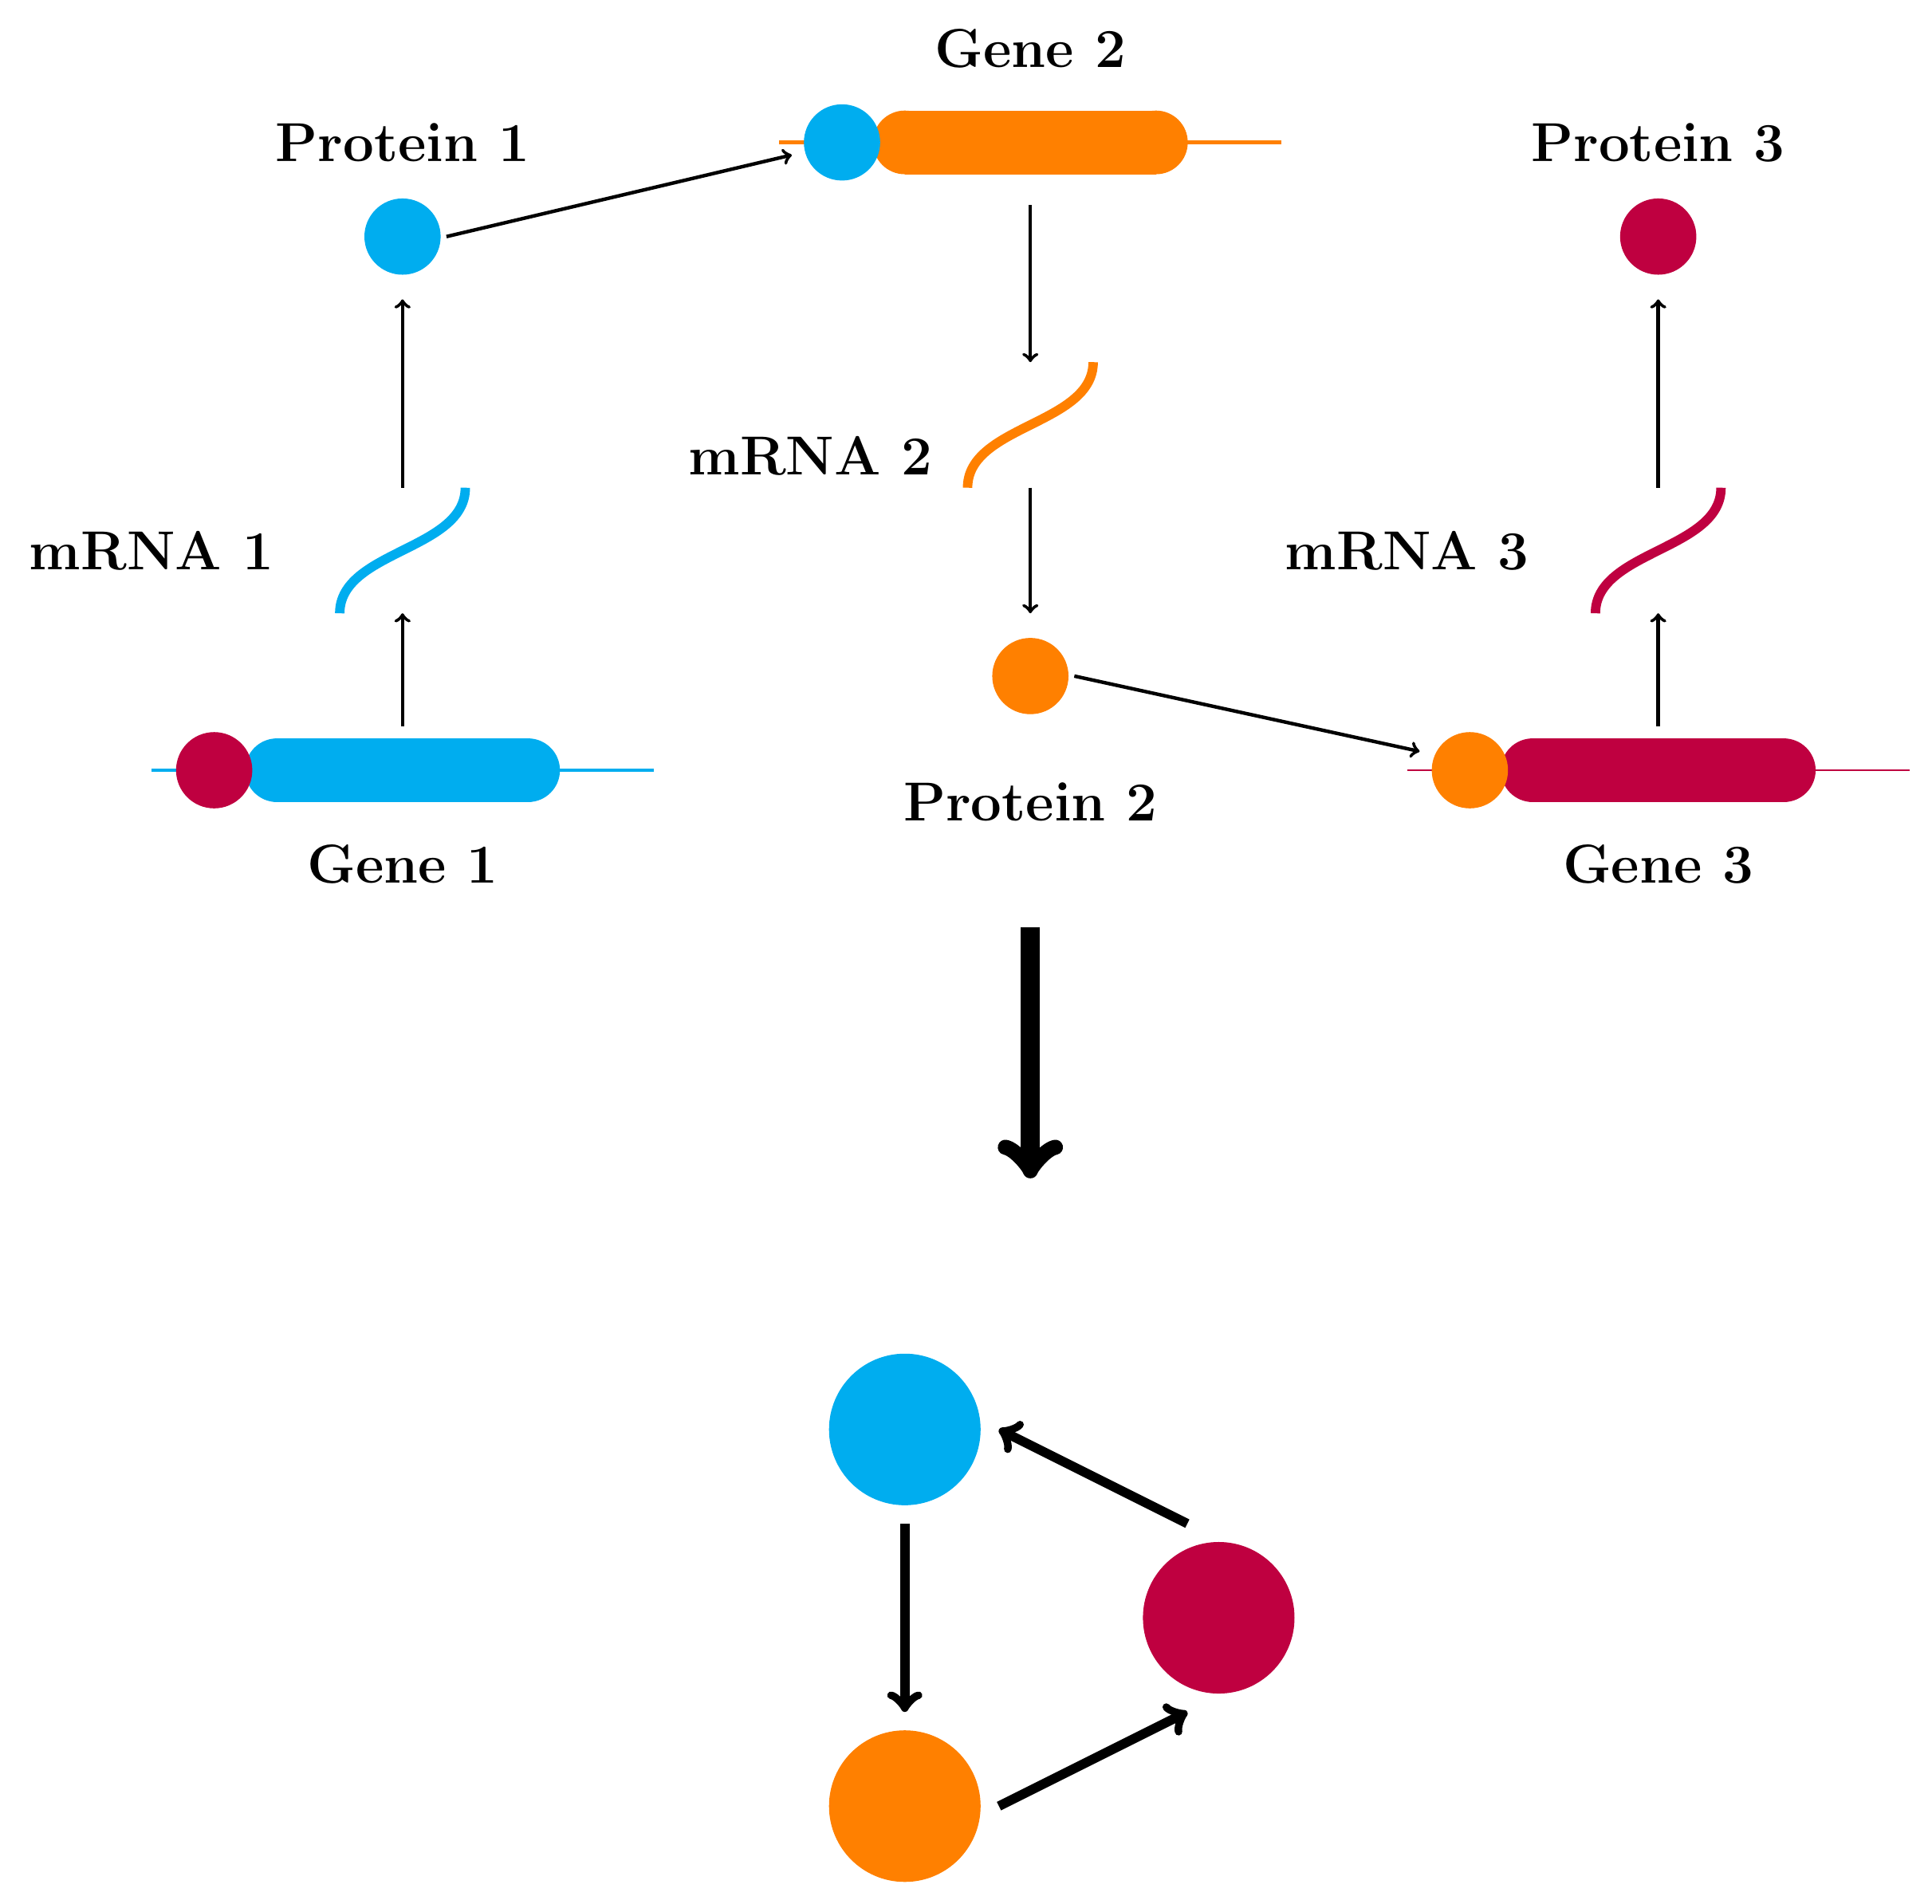
\begin{tikzpicture} [scale=1]

\draw[fill,orange] (10,10) -- (14,10) -- (14,11) -- (10,11) --(10,10);
\draw [fill,orange] (10,10.5) circle (0.5cm);
\draw [fill,orange] (14,10.5) circle (0.5cm);
\draw [orange,ultra thick] (8,10.5) -- (16,10.5);
\draw [->, ultra thick] (12.,9.5) -- (12.,7);
\draw [orange,ultra thick,line width=0.15cm] (11.,5.) .. controls (11.,6.) and (13.,6.) .. (13.,7.);
\draw [fill, orange] (12.,2) circle (0.6cm);
\draw [->, ultra thick] (12.,5) -- (12.,3);




\draw[fill,cyan] (0,0) -- (4,0) -- (4,1) -- (0,1) --(0,0);
\draw [fill,cyan] (0,0.5) circle (0.5cm);
\draw [fill,cyan] (4,0.5) circle (0.5cm);
\draw [cyan,ultra thick] (-2,0.5) -- (6,0.5);
\draw [->, ultra thick] (2,1.2) -- (2,3);
\draw [cyan,ultra  thick,line width=0.15cm] (1,3) .. controls (1,4) and (3,4) .. (3,5);
\draw [->, ultra thick] (2,5) -- (2, 8);
\draw [fill, cyan] (2,9) circle (0.6cm);

\draw [fill, cyan] (9,10.5) circle (0.6cm);
\draw[->, ultra thick] (2.7,9) -- (8.2,10.3);

\draw[fill,purple] (20,0) -- (24,0) -- (24,1) -- (20,1) --(20,0);
\draw [fill,purple] (20,0.5) circle (0.5cm);
\draw [fill,purple] (24,0.5) circle (0.5cm);
\draw [purple] (18,0.5) -- (26,0.5);
\draw [->, ultra thick] (22,1.2) -- (22,3);
\draw [purple,ultra  thick,line width=0.15cm] (21,3) .. controls (21,4) and (23,4) .. (23,5);
\draw [->, ultra thick] (22,5) -- (22, 8);
\draw [fill, purple] (22,9) circle (0.6cm);


\draw [fill, orange] (19.,0.5) circle (0.6cm);
\draw[->,ultra thick] (12.7,2) -- ( 18.2,0.8);

\draw [fill, purple] (-1.,0.5) circle (0.6cm);


\node at (2,-1) {\Huge{\textbf{Gene 1}}};
\node at (12,12) {\Huge{\textbf{Gene 2}}};
\node at (22,-1) {\Huge{\textbf{Gene 3}}};

\node at (-2,4) {\Huge{\textbf{mRNA 1}}};
\node at (8.5,5.5) {\Huge{\textbf{mRNA 2}}};
\node at (18,4) {\Huge{\textbf{mRNA 3}}};

\node at (2,10.5) {\Huge{\textbf{Protein 1}}};
\node at (12,0) {\Huge{\textbf{Protein 2}}};
\node at (22,10.5) {\Huge{\textbf{Protein 3}}};


\draw[->,line width = 0.3cm] (12,-2) -- (12,-6);

\draw[fill,cyan] (10,-10) circle (1.2cm); 
\draw[fill,orange] (10,-16) circle (1.2cm); 
\draw[fill,purple] (15,-13) circle (1.2cm); 
\draw[->, line width = 0.15cm] (10,-11.5) -- (10,-14.5);
\draw[->, line width = 0.15cm] (11.5,-16) -- (14.5,-14.5);
\draw[->, line width = 0.15cm] (14.5,-11.5) -- (11.5,-10);


\end{tikzpicture}
\end{document}
